% Template from the DPHPC course website

% IEEE standard conference template; to be used with:
%   spconf.sty  - LaTeX style file, and
%   IEEEbib.bst - IEEE bibliography style file.
% --------------------------------------------------------------------------

\documentclass[letterpaper]{article}
\usepackage{spconf,amsmath,amssymb,graphicx}
\usepackage[english]{babel}
\usepackage[utf8]{inputenc}
\usepackage{verbatim}		
\usepackage{epstopdf}
\usepackage[font=footnotesize]{caption}
\usepackage[dvipsnames]{xcolor}
\usepackage{hyperref}
\usepackage{listings}	
\usepackage{multicol}
\usepackage{ifthen}
\usepackage{tikz}
\usepackage{placeins}
\usetikzlibrary{arrows,decorations.pathmorphing,backgrounds,fit,positioning,shapes.symbols,chains,calc,shapes}

\usepackage[ruled,noend,noline,slide]{algorithm2e}
\newenvironment{listing}[1][htb]
  {\renewcommand{\algorithmcfname}{Listing}% Update algorithm name
   \begin{algorithm}[#1]%
  }{\end{algorithm}}

\usepackage{booktabs}
  
% Example definitions.
% --------------------
% Nice typeset for C++
\newcommand{\Cpp}{C\nolinebreak[4]\hspace{-.05em}\raisebox{.2ex}{\small \bf ++}}
%\newcommand{\Cpp}{C\nolinebreak\hspace{-.05em}\raisebox{.4ex}{\tiny\bf +}\nolinebreak\hspace{-.10em}\raisebox{.4ex}{\tiny\bf +}}
%\newcommand{\Cpp}{\texttt{C\nolinebreak+\nolinebreak+}}


% bold paragraph titles
\newcommand{\mypar}[1]{{\bf #1.}}

\ifthenelse{\boolean{true}}% TODO: change to false to hide invisible notes
{ \newenvironment{invisible}{\par\bigskip\color{gray}}{\par\bigskip} }%
{ \newenvironment{invisible}{\expandafter\comment}{\expandafter\endcomment} }

\title{Topological Sorting: A Parallel Implementation}

\name{J. Baum, K. Wallimann, M. Untergassmair}%
\address{ETH Zürich, HS 2015 \\
	Design of Parallel and High Performance Computing \\
	Zürich, Switzerland}

%%%%%%%%%%%%%%%%%%%%%%%%%%%%%%%%%%%%%%%%%%%%%%%%%%%%%%%%%%%%%%%%%%%%%%%%%%%%%%%%

\begin{document}

\maketitle

\begin{abstract}
	This short report gives a quick insight in topological sorting and the various problems that are associated with its parallelization.
	Building on existing algorithms, it suggests modified and optimized approaches to overcome these problems while making best use of state of the art computer hardware.
	In a discussion of the obtained benchmarks the performance of these approaches is analyzed and compared.
	Lastly, this report contains some suggestions regarding which graph types might profit from parallel topological sorting.
\end{abstract}

\section{Introduction}\label{sec:intro}

\mypar{Motivation}
\begin{invisible}
  \begin{itemize}
  \item Software Dependencies
  \item Maybe, to flesh out: Admittedly a bit academic, but interesting problem nevertheless, because memory bound => This is the future of HPC
  \end{itemize}
\end{invisible}


\mypar{Related work} 
\begin{invisible}
  \begin{itemize}
  \item MC Er Paper \cite{er1983parallel}: Unclear how to retrieve a sorted list from values without sorting and threads might chase other threads. No words about load balancing => Not practicable
  \item Ma Paper \cite{ma1997efficient}: Theoretical analysis in PRAM model, not practicable.
  \item Both cases: No code
  \item Our contribution: (1) Modified algorithm based on MC Er. 1. Sorted list is directly extracted. 2. only one thread continues when multiple threads meet. 3. Ensure load balancing
                          (2) Actual implementation for shared memory architecture
  \end{itemize}
\end{invisible}



\section{Algorithm}\label{sec:background}
%TODO: Johannes

 In this section, we define the topological sort problem and contrast it to Breadth-First-Search (BFS) and Depth-First-Search (DFS).
 Furthermore, we introduce the basics of the parallel algorithm we use.
 \\
 

\mypar{Topological sorting}
 A directed acyclic graph (DAG) describes a partial order. A topological sorting is a total order on a DAG. Let $G = (V,E)$ be a DAG where $V$ is the set of vertices and $E$ is the set of edges. Formally a topological sorting is a function $ord: V \longrightarrow \{1,...,n\}$ where $n = |V|$ such that $\forall (v,w) \in E: ord(v) < ord(w)$ \cite[Chapter~9.1]{ottmann2012algorithmen}.
\begin{invisible}
Herausfinden, ob ord(v) < ord (w) oder $\leq$. Citation! Widmayer?
\end{invisible}

Figure \ref{fig:ts-example} shows a DAG with a corresponding topological sorting: A,I,F,B,E,D,H,G,C. Even though every DAG has at least one topological sorting, in general there are many different topological sortings for the same graph.

\begin{figure}[!hbp]
 \centering
  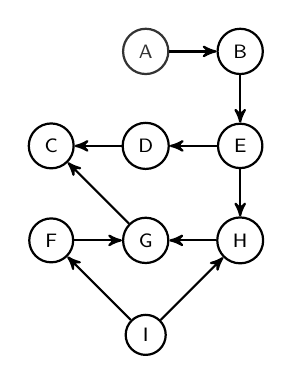
\begin{tikzpicture}[->,>=stealth',auto,node distance=1cm,
                    thick,main
                    node/.style={circle,draw,font=\sffamily\scriptsize},text node/.style={draw=none,font=\sffamily\tiny}]

  \node[main node] (1) [draw=black!80,text=black!80] {A};
  \node[main node] (3) [right of=1, node distance=1.2cm]{B};
  \node[main node] (7) [below of=3, node distance=1.2cm] {E};
  \node[main node] (4) [left of=7, node distance=1.2cm] {D};
  \node[main node] (5) [below of=7, node distance=1.2cm] {H};
  \node[main node] (6) [left of=4, node distance=1.2cm] {C};
  \node[main node] (8) [left of=5, node distance=1.2cm] {G};
  \node[main node] (9) [below of=8, node distance=1.2cm] {I};
  \node[main node] (2) [left of=8, node distance=1.2cm] {F};


  \path[every node/.style={font=\sffamily\small}]
    (1) edge (3)
    (3) edge (7)
    (7) edge (4)
    (4) edge (6)
    (7) edge (5)
    (5) edge (8)
    (8) edge (6)
    (9) edge (5)
    (9) edge (2)
    (2) edge (8)
    ;
\end{tikzpicture}

\caption{Example DAG where A,I,F,B,E,D,H,G,C is one possible topological sorting}
\label{fig:ts-example}
\end{figure}

Topological sortings can be  used to schedule tasks based on their dependencies. Every vertex represents a task and the edges represent the relation between the tasks.

Although the results of the breadth-first-search (BFS) algorithm seem to be similar to topological sortings, they are not equivalent. The difference between the results of BFS and a topological sorting is, that a topological sorting is a total order with respect to the partial order represented by the input graph. In contrast, the traversal sequence of a BFS (and DFS) generally don’t correspond to a total order induced by a DAG. A simple example is shown in figure \ref{fig:diff-bfs}. The visiting sequence A,C,B is valid in BFS but is not a topological sorting. The only valid topological sorting for the example graph is A,B,C.


\begin{figure}[!hbp]
\centering
 
  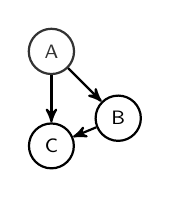
\begin{tikzpicture}[->,>=stealth',auto,node distance=1cm,
                    thick,main
                    node/.style={circle,draw,font=\sffamily\scriptsize},text node/.style={draw=none,font=\sffamily\tiny}]

  \node[main node] (1) [draw=black!80,text=black!80] {A};
  \node[main node] (2) [below right of=1, node distance=1.2cm]{B};
  \node[main node] (3) [below of=1, node distance=1.2cm] {C};
 

  \path[every node/.style={font=\sffamily\small}]
    (1) edge (2)
    (2) edge (3)
    (1) edge (3)
    ;
\end{tikzpicture}

\caption{A,C,B is a valid sequence in breadth-first-search (BFS) and depth-first-search (DFS) but not a topological sorting}
\label{fig:diff-bfs}
\end{figure}

A sequential algorithm yielding a topological sorting has been suggested by Kahn \cite{kahn1962topological}. Another algorithm has been published by Tarjan  \cite{tarjan1976edge} and is based on a DFS with backtracking. Topological sorting has an asymptotic complexity of $\mathcal{O}(|V|+|E|)$ \cite[Chapter~22.4]{cormen2001introduction}. 

 \mypar{Parallel algorithm}
 In 1983 M. C. Er \cite{er1983parallel} came up with a parallel approach to retrieve a topological sorting. The algorithm works in 5 steps:
 \begin{enumerate}
        \item Build the graph from the given partial order (optional if the problem is already stated as a graph).
        \item Add a special node value to every node and initialize it to zero
        \item Visit all source nodes (nodes with an indegree of zero) and set their node values to one.
        \item Start from all source nodes in parallel and proceed for all successor nodes as follows: Let $N_p$ be the node value of the current source node and $N_s$ the node value of the currently observed successor node. Then the algorithm checks if $N_s \leq N_p$ and sets the value of the successor to $N_p + 1$, if so. This step is iterated until there are no further successor nodes. 
        \item List all the nodes in ascending order of node values.
 \end{enumerate}

To avoid a race condition by concurrent writes to a node’s value, M. C. Er proposes a synchronization after every step. Therefore, any two threads would write the same number to a node’s value, because the barrier ensures that all threads are in the same step. This comes at the price of a lower performance. Node values might be rewritten by multiple threads that "follow" each other. For example, in figure \ref{fig:ts-example}, node H, G and C could receive the values 2,3,4 initially, but would eventually be overwritten with the values 4,5,6


The asymptotic parallel runtime of the above algorithm is described by M. C. Er as $\mathcal{O}(D_{max})$, where $D_{max}$ is defined as the maximum distance between a source node and a sink node. This runtime is hard to achieve in practice if one implements step 5 of the algorithm via sorting the nodes with respect to their values. It is not mentioned by M. C. Er how to create the result list of step 5.


\mypar{Improvements}
We propose not to use node values, but to directly put the node into the solution list. This avoids sorting the nodes by their value at the end. Also the barriers are not necessary anymore. However, it must be made sure that no node is written more than once to the result list and race conditions while writing to the solution list must be avoided.

Furthermore, we introduce a parent counter to address the problem of several processes following the same path. The parent counter is initialized to the number of parent nodes. During the algorithm each thread arriving at a node will decrease the counter by one. It will only process the node if the parent counter is zero. Thus a node will be processed only by the last arriving thread. It has to be taken care of the race condition while updating the parent counter.



 
 
 
 \begin{invisible}
 % Serial TS
 \mypar{Topological sorting}
 \begin{itemize}
  \item What is topological sort, difference to BFS
  \item Input: A set of dependencies (aka partial orders) of the form A $\rightarrow$ B ``A must come before B''
  \item Output: A sequence (aka total order) containing all nodes exactly once. All partial orders must be kept.
  \item Solution not unique
  \item Minimal Example: A->B, A->C, B->C. Valid BFS traversal order: A, C, B. Invalid for TS.
  \item TS can (serially) be solved with Kahn's algorithm \cite{kahn1962topological} or DFS and Backpropagation (Tarjan \cite{tarjan1976edge}). % See Wikipedia
        Note that TS is not equivalent to DFS, e.g. for A->B, B->C, A->D, D->E, DFS and Backpropagation yields A, B, C, D, E, but another valid TS is A, B, D, C, E
  \item Asymptotic runtime: O(|V| + |E|)
As an aside, don't talk about "the complexity of the algorithm.'' It's incorrect,
problems have a complexity, not algorithms.  
 \end{itemize}

 % Multithreaded TS
 \mypar{Parallel algorithm}
 \begin{itemize}
  \item Short overview over algorithm of MC Er
  \item Parallelization over child nodes
  \item His idea with barrier in each step such that even if the index is written by multiple threads, they write the same number => Avoid race condition at writing the index
  \item Our idea: Instead of writing an index, directly write to solution list. As a consequence, we have to make sure that node is written to solution only once. And of course there is a race condition on writing to solution list.
  \item Our idea: First, count (in parallel) how many parents each node has. Each time a node is visited, decrement counter and only write to solution if counter is zero. Of course, there is a race condition on the parent counter.
  \item 3 synchronization points (that is, bottlenecks): 1. Barrier after each level, 2. Lock solution list for appending new nodes, 3. Lock parent counter for decrementing it and checking if it is zero.
  \item Cost
 \end{itemize}

 
\end{invisible}

%TODO: Change title
\section{Efficient parallel implementation}\label{sec:yourmethod}
%TODO: Kevin
%TODO: Somewhere, we must state the problem: Input many partial orderings, Output one total order (a solution list)

In this section, the implementation of the parallel algorithm outlined above is presented.
Especially, we show how to ensure load balancing, how to efficiently handle appending nodes to the solution list, decrementing and checking the parent counter, and how to circumvent barriers.

\mypar{Parallelization and load balancing}
Parallelization is achieved by distributing the nodes in the current front among the threads. We experimented with two representations of the front.

Firstly, we implemented the front using thread-local lists, following an idea described in \cite{bulucc2011parallel}.
The nodes in the front are split among the threads, such that each thread owns a thread-local list, from which it processes the nodes in the current front.
Child nodes for the next front are first inserted to another thread-local list.
When the whole front was processed, one thread collects all thread-local lists and redistributes the new child nodes among the threads.
Redistribution for each front already yields some level of load balancing.
A further refinement of load balancing was implemented by using a work stealing policy.
If one thread runs out of nodes within a front, it can steal nodes from another thread that has not finished yet.

Secondly, we implemented the front using a bitset, like in \cite{agarwal2010scalable} or \cite{beamer2013direction}. The size of the bitset is equal to the number of nodes.
The last parent visiting a child node sets the child nodes' bit to true. Parallelization is then enabled by parallelizing the loop over the bitset.
Load balancing is conveniently achieved using a dynamic scheduler.
Notice that we actually refer to an array of booleans when using the term bitset. A space-efficient bitset is not thread-safe.


\mypar{Efficient appending to the solution list}
The algorithm proceeds front by front.
%All nodes in the current front have already been visited by all their parent nodes. % This is actually an invariant, but never mind.
%This is ensured by admitting only those child nodes to the next front, for which the current node is the last visiting parent node. % Maybe belongs to algorithm description
Nodes in the current front are ready to be inserted to the global solution list.
Since all nodes in the current front have been visited by all of their parent nodes, one node cannot be a parent of another node in the current front.
Therefore, the order among the nodes on one front does not matter for the topological sorting.
As a consequence, the nodes can be appended to the solution in parallel without any restrictions on the order.
Still, the solution list has to be locked for every appending of a node, which is not optimal.

The optimization that is proposed here is simple: Every thread first inserts the nodes in a thread-local list and then appends the whole local list to the solution list.
Thereby, each thread grabs the lock only once per front and not for every node individually.
For lists, appending another list can be done in constant time.

\mypar{Efficiently decrementing and checking the parent counter}
In the parallel algorithm, every node has a parent counter that is initialized with the number of parent nodes.
As explained before, a node may only be inserted if all its parents have visited it.
Therefore, each parent has to decrement the parent counter to mark its visit and it has to check whether the parent counter is zero, i.e. whether it is the last visiting parent.
Na{\"i}vely, the decrement and the check have to be locked together, in order to avoid race conditions on the counter on the one hand, and in order to ensure that only one thread may return true on the other hand. 
However, a closer examination reveals that these requirements can be met by using atomic operations.

\begin{listing}
 \SetKw{KwRet}{Return}
 \SetKw{KwBool}{Bool}
 \SetKw{KwInt}{Integer}
 \SetKwProg{Fn}{Function}{}{}
  \KwInt parentCounter\;
  \tcp{initialized with number of parent nodes}
  \KwBool token = false\;
  \Fn{decrementAndCheckParentCounter{}} {
    AtomicDecrement(parentCounter)\;
    \KwBool swapped = false\;
    \If{parentCounter == 0}{
      swapped = AtomicCompareAndSwap(token, false, true)\;
    }
    \KwRet swapped;
  }
 \caption{Efficiently decrementing and checking the parent counter using atomics.}
 \label{lst:parentCounter}
\end{listing}

Listing \ref{lst:parentCounter} shows the implementation using atomic operations. Multiple threads may in fact decrement the counter before the function returns.
However the atomic compare-and-swap ensures that only one thread can return true. This is important if the current front is implemented as a list.
In this case, the child node would be inserted twice, if multiple threads returned true, which is wrong.
If the front is implemented as a bitset, the compare-and-swap is in fact not necessary, because it makes no difference if multiple threads set the bit.

\mypar{Barrier-free implementation}
Barriers were used to process the nodes in a front-by-front fashion.
Each front is finished with a barrier, either explicitly, if the front was implemented with a list, or implicitly by a for-loop, if the front was implemented using a bitset.

If barriers are given up, it is no longer certain that all threads work on nodes of the same front.
Some threads may already work on nodes of the next front, while other threads are still working on the previous front.

A priori, this is not a problem, because in any case, a node is only appended to the solution list if all its parents have visited it, regardless of which front its parents belonged to.
However, it is not possible to temporarily store a node in a thread-local list and defer the appending to the solution list, as suggested earlier.
In this case, it would be possible that a node was appended to the solution list, while its parent node has only been appended to a thread-local list, but not yet to the solution list, leading to a invalid result.

Hence, avoiding barriers seems to be a trade-off between the cost of barriers and the cost of locking the solution list for every node.

\begin{invisible}
Hmm... we could defer decrementing the parent counter and inserting the child node until the local list is appended to the solution list. That means, that we have to touch all nodes twice
Somewhere, we need to mention that we are working with an adjacency list.
\end{invisible}
\section{Experimental Results}\label{sec:exp}
%
In this section, we present our experimental setup and the impact of the different optimizations and implementations described in the previous section.
\par\medskip
%
\begin{invisible}
	Ist wahrscheinlich doch keine Gute Idee, das Abstiming zu plotten - die Schnellen Algorithmen haben fast identische laufzeiten und die anderen sind seeeeeeeeeehr schlecht
\end{invisible}
%
\mypar{Dependency on Graph Type} Before discussing the differences between the algorithms that we implemented, we want to have a closer look at the input graphs.
Figure \ref{fig:strongscaling_graphtypes} shows the strong scaling of the BITSET algorithm for several different input graphs:
The multichain graphs consist of multiple chains of length 100 and 1000 respectively, \ldots and the software graph was constructed accorting to \ldots \\
\begin{invisible}
	{\Large TODO:} quick description of graphs here
\end{invisible}
It should be noted at this point that all of the analyzed graphs are artificial (i.e. they do not come from real-world datasets but are rather constructed to meet some requirements).
The DAGs we used for our analysis are sparse, meaning that the number of edges $|E|$ in the graph is much smaller than the maximum number of vertices $|V|\cdot(|V|-1)$ and in particular that the number of edges in the graph scale linearly with the graph size, $|E| \sim \mathcal{O} ( |V| )$. \\
It can be expected that the following performance analysis based on artificial graphs is a good indicator of how the presented topological sorting algorithms would scale for real-world graphs with similar parameters.
To this point however, the performance of the algorithms on real-world graphs was not tested yet, and an investigation of such could be content of further research.
\par\medskip
%
For the remaining performance analysis, only the random graph with node degree 16 is considered.
Plots for other graph types can be found in the repository of our project which is listed at the end of this report.

% \begin{figure}[ht]
% 	\centering
% 	\includegraphics[width=\columnwidth]{plots/abstiming_gtRANDOMLIN_n1000000_deg16.pdf}
% 	\caption{<+caption text+>}
% 	\label{fig:<+label+>}
% \end{figure}
 
\begin{figure}[ht]
	\centering
	\includegraphics[width=\columnwidth]{plots/strongscaling_gtALL_n1000000.pdf}
	\caption{<+caption text+>}
	\label{fig:strongscaling_graphtypes}
\end{figure}
 
\begin{figure}[ht]
	\centering
	\includegraphics[width=\columnwidth]{plots/strongscaling_gtRANDOMLIN_n1000000_deg16.pdf}
	\caption{<+caption text+>}
	\label{fig:<+label+>}
\end{figure}
 
\begin{figure}[ht]
	\centering
	\includegraphics[width=\columnwidth]{plots/weakscaling_gtRANDOMLIN16_n1000000_deg16.pdf}
	\caption{<+caption text+>}
	\label{fig:<+label+>}
\end{figure}



\mypar{Hardware and compiler}
  \begin{table}[h]
    \centering
    \begin{tabular}{ll}
    \toprule
    Processor        & Intel Xeon E5-2697 (Ivy bridge) \\
    Max. clock rate  & 3.5 GHz (with TurboBoost)\\
    \# Sockets       & 2 \\
    Cores / socket   & 12 \\
    Threads / socket & 24 \\
    LLC / socket     & 30 MB \\
    \midrule
    Compiler and flags & GCC 4.8.2, -O3\\
    \bottomrule
    \end{tabular}
    \caption{Hardware and compiler used for benchmarks}
    \label{tab:hardware}
  \end{table}
 
 The following experiments were run on a 24-core system consisting of 2 Intel Xeon E5 processors (see table \ref{tab:hardware}).
 Hyperthreading was not used for the benchmarks.
 The implementations were written in \Cpp, using OpenMP and GCC atomic built-in functions. The graph was stored in an adjacency list.
\begin{invisible}

 \mypar{Benchmarks}
 For each item, mention graph type, number of nodes, node degree, optimizations from above
 \begin{itemize}
  \item Influence of barrier. Introduce multichain graph, Strong Scaling dynamic nobarrier opt2 MULTICHAIN100 vs bitset global opt1 MULTICHAIN100 Why Multichain100: Should be dominated by barrier%bitset_global is bitset without local solutions, because dynamic_nobarrier has no local solutions
  \item Influence of local solution. Strong Scaling bitset MULTICHAIN10000 vs bitset global MULTICHAIN10000 Why Multichain10000: Should be dominated by pushbacks to solution
  \item Influence of atomic counter check. Strong Scaling RANDOMLIN 100000 opt = true vs opt = false for worksteal and bitset
  \item Strong Scaling software graph \cite{musco2014generative}
  \item Strong Scaling random graph with different degrees
  \item Vertex Scaling plot random graph
 \end{itemize}

\mypar{Results}

Questions to each plot
\begin{itemize}
 \item What is the performance penalty of the barrier?
 \item How well performs the local solution compared to locking the 
 \item How does the atomic counter check scale compared to the locked version?
 \item How does the best version of our code scale on a real-world example?
 \item How does the best version of our code scale in a slightly artificial scenario?
\end{itemize}
\end{invisible}

\section{Conclusion}
%
In this report we have extended the theoretical considerations made in \cite{er1983parallel} and discussed as well as tested its parallel implementation.
Both the Worksteal and the Node-Lookup approach can be considered successful parallelizations of the topological sorting algorithm, with the latter showing better absolute timings and scaling behavior for the graphs that were analyzed. \\
Finally, one main finding of this project is that the efficiency of the parallelization highly depends on the graph type: if the graph is too sparse and each node has only very few outgoing edges, then the parallelizable portion of the algorithm shrinks and by Amdahl's law the synchronization overhead dominates the runtime resulting in bad scaling. \\

\begin{invisible}
 \begin{itemize}
   \item Best thing would be to have no barriers and still local solution update
   \item Since this is not possible, it is better to accept barriers so as to benefit from local solution
   \item It is worth noting that performance highly depends on the structure of the graph.
 \end{itemize}
\end{invisible}


\section{Additional material}
%
The source code of the project, a database containing all the raw data that was collected for the benchmarking plots as well as many more detailed plots depicting the scaling behavior for all tested graph types can be found in the following Git repository:
\begin{center}
	\href{https://github.com/walkevin/ParallelTopologicalSorting.git}{https://github.com/walkevin/ParallelTopologicalSorting.git}
\end{center}


\bibliographystyle{IEEEbib}
\bibliography{bibliography}

\end{document}
